\chapter{Experiments}

In the following sections we discuss a series of experiments relating to the methods discussed above. 
We first introduce some experiment using simulated data, where we can verify and compare the results with a known distribution.
We then discuss some experiments relating to improving the SGHMC through better estimation of the variance $\hat{V}$.
Finally, we apply the methods discussed to some deep learning problems using the MNIST and CIFAR10 datasets.

\section{Simulated data}

In order to verify the implementation of the MCMC methods, we carry out some simulation experiments.
The first experiment is a recreation of an experiment also carried out in the SGHMC paper, where they sample from a bimodal distribution with $\log p(x) \propto 2 x^2 - x^ 4$ with different configurations. 
First, the distribution is sampled from as is, using regular HMC.
Then the batched dynamics in \cref{eq:sghmc-model} are simulated by adding simulated noise $\epsilon \sim \mathcal{N}(0, 4)$ to the gradient during the sampling process. 
The distributional assumptions of SGHMC are thus fulfilled exactly, and we may also use the known noise scale as the noise estimate for SGHMC. 
With this introduced noise we also investigate the naive approach to using HMC, both with and without using an MH step. 
The resulting sampled distributions can be seen in \cref{fig:synthetic}
\begin{figure}[htb]
    \centering
    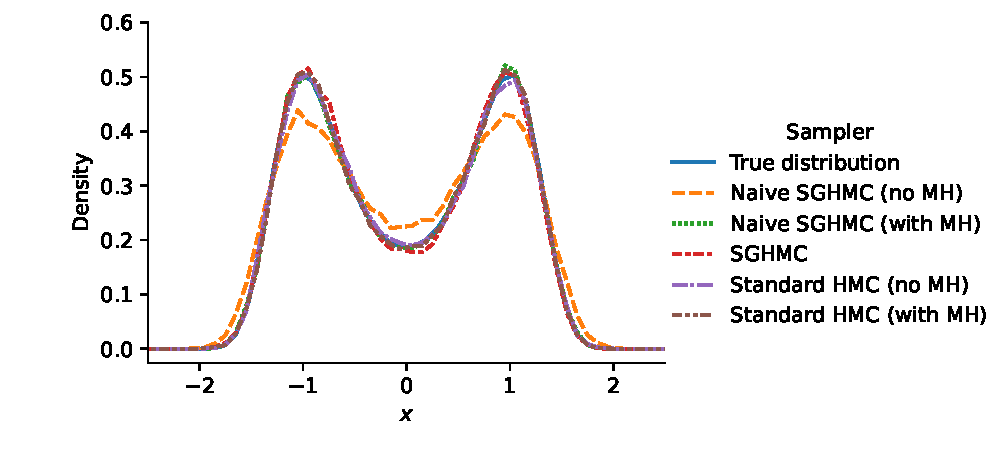
\includegraphics[width=0.9\textwidth]{Figures/synthetic.pdf}
    \caption{Samples from $\log p(x) \propto 2 x^2 - x^ 4$ for different sampling configurations}
    \label{fig:synthetic}
\end{figure}
These result seem to verify our that our implementation is correct.
We also see that the sample distributions from both the standard HMC sampler and the SGHMC sampler closely resembles the true distribution. 
The naive SGHMC sampler does seems to break down when no MH step is included, and since we also compare with regular HMC with no MH step, this demonstrates that it may not be purely down to omitting the MH step. 

If we include an MH step, the naive approach also seem to work, however we are not adding any noise to $E(\cdot)$ when performing the MH step, corresponding to calculating $E(\cdot)$ across the whole data set. 
This is impractical in the context of deep learning, but one could imagine an alternative naive HMC approach where an MH step based on each individual batch of data. 

This experiment also doesn't address whether noise the dynamics of \cref{eq:sghmc-model} are even reasonable as a model for the noise introduced through batching the gradient. 

In order to address these points, we perform an additional simulation experiment. 
This is also to demonstrate the relevance of the different methods in the context of MCMC inference.
We consider the polynomial model of $P(x) = -x + \frac{1}{2}x^2 + \frac{1}{3}x^3$, 
and with $\epsilon \sim \mathcal{N}(0, 1)$, consider a set learning points $y_i = P(x_i) + \epsilon$ for $i=1,\dots,15$, where $x_i$ are linearly spaced over the interval $[-3, 3)$ with a small amount of noise added. 
We then consider the problem of bayesian polynomial regression with known noise $\sigma=1$ and the regression model:
\begin{align*}
    P(x) = a_0 + a_1 x+a_2 x^2 + a_3 x^3
\end{align*}
where each parameter are given a $\mathcal{N}(0, 1)$ prior.
The exact parameter posterior $p(a|x,y)$ for this regression problem is known, and can therefore be compared to the sampled distribution of the samplers. 
More specifically, three sampling strategies are considered, regular HMC conditioned on all data points, HMC where each sample is based on a batch of 5 observations, and SGHMC also with batches of 5 observations.
For demonstration, a plot of the sampled joint distribution of $a_1$ and $a_3$ can be seen in \cref{fig:simulated_joint_comp}.
\begin{figure}[htbp]
    \centering
    \begin{subfigure}[b]{0.45\linewidth}
        \centering
        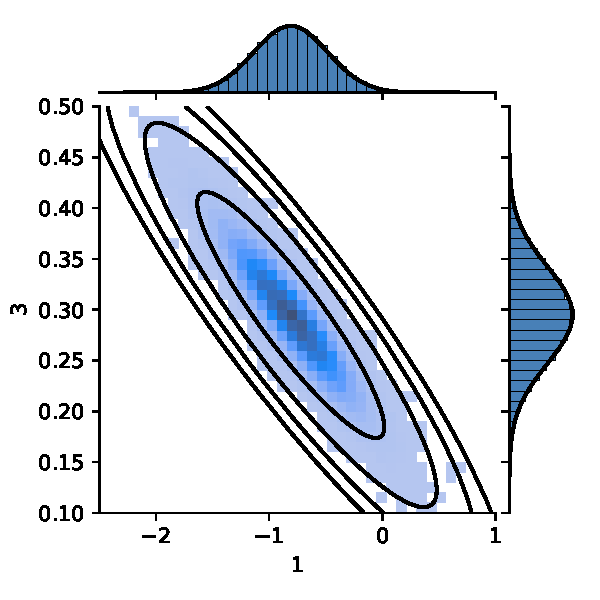
\includegraphics[width=\linewidth]{Figures/simulated_joint_HMC_15.pdf} 
        \caption{HMC conditioned on all data points.}
    \end{subfigure}
    \begin{subfigure}[b]{0.45\linewidth}
        \centering
        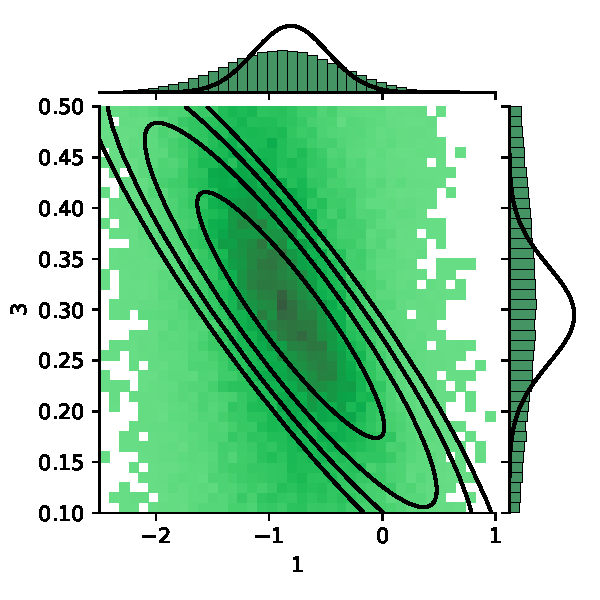
\includegraphics[width=\linewidth]{Figures/simulated_joint_HMC_5.pdf} 
        \caption{HMC with batch size 5}
    \end{subfigure}
    \begin{subfigure}[b]{0.45\linewidth}
        \centering
        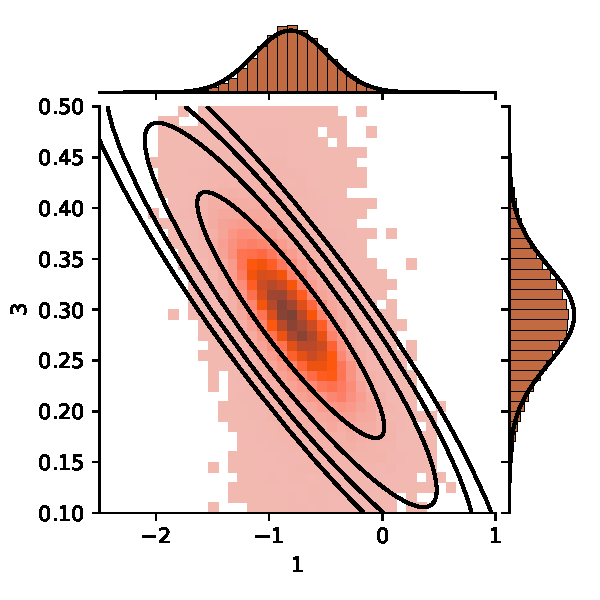
\includegraphics[width=\linewidth]{Figures/simulated_joint_SGHMC_5.pdf} 
        \caption{SGHMC with batch size 5}
    \end{subfigure}
    \caption{Joint distribution of samples for $a_1$ and $a_3$ for the polynomial regression example for HMC and SGHMC for different batch sizes, with the actual posterior density also shown.}
    \label{fig:simulated_joint_comp}
\end{figure}
We find that the also with this approach to the naive SGHMC the batched HMC doesn't, with the sampled posterior having 

with not even the marginal densities being anywhere close to the actual parameter posterior.
Notably, the SGHMC seems to provide a more reasonable estimate, however still with some overdispersion.
In the following section, a possible improvement upon this algorithm is discussed.

\subsection{Variational Inference} 
We can also repeat the experiment above using the variational inference framework.
A comparison of the pairwise marginal distributions for the true posterior and the variational posterior can be seen in \cref{fig:vi-simulated}. 
Since we are assuming independent variables for the variational posterior, the fit is not particular good compared to the MCMC methods. 
However, this still serves to verify that the implementation is behaving as expected.
\begin{figure}[htbp]
    \centering
    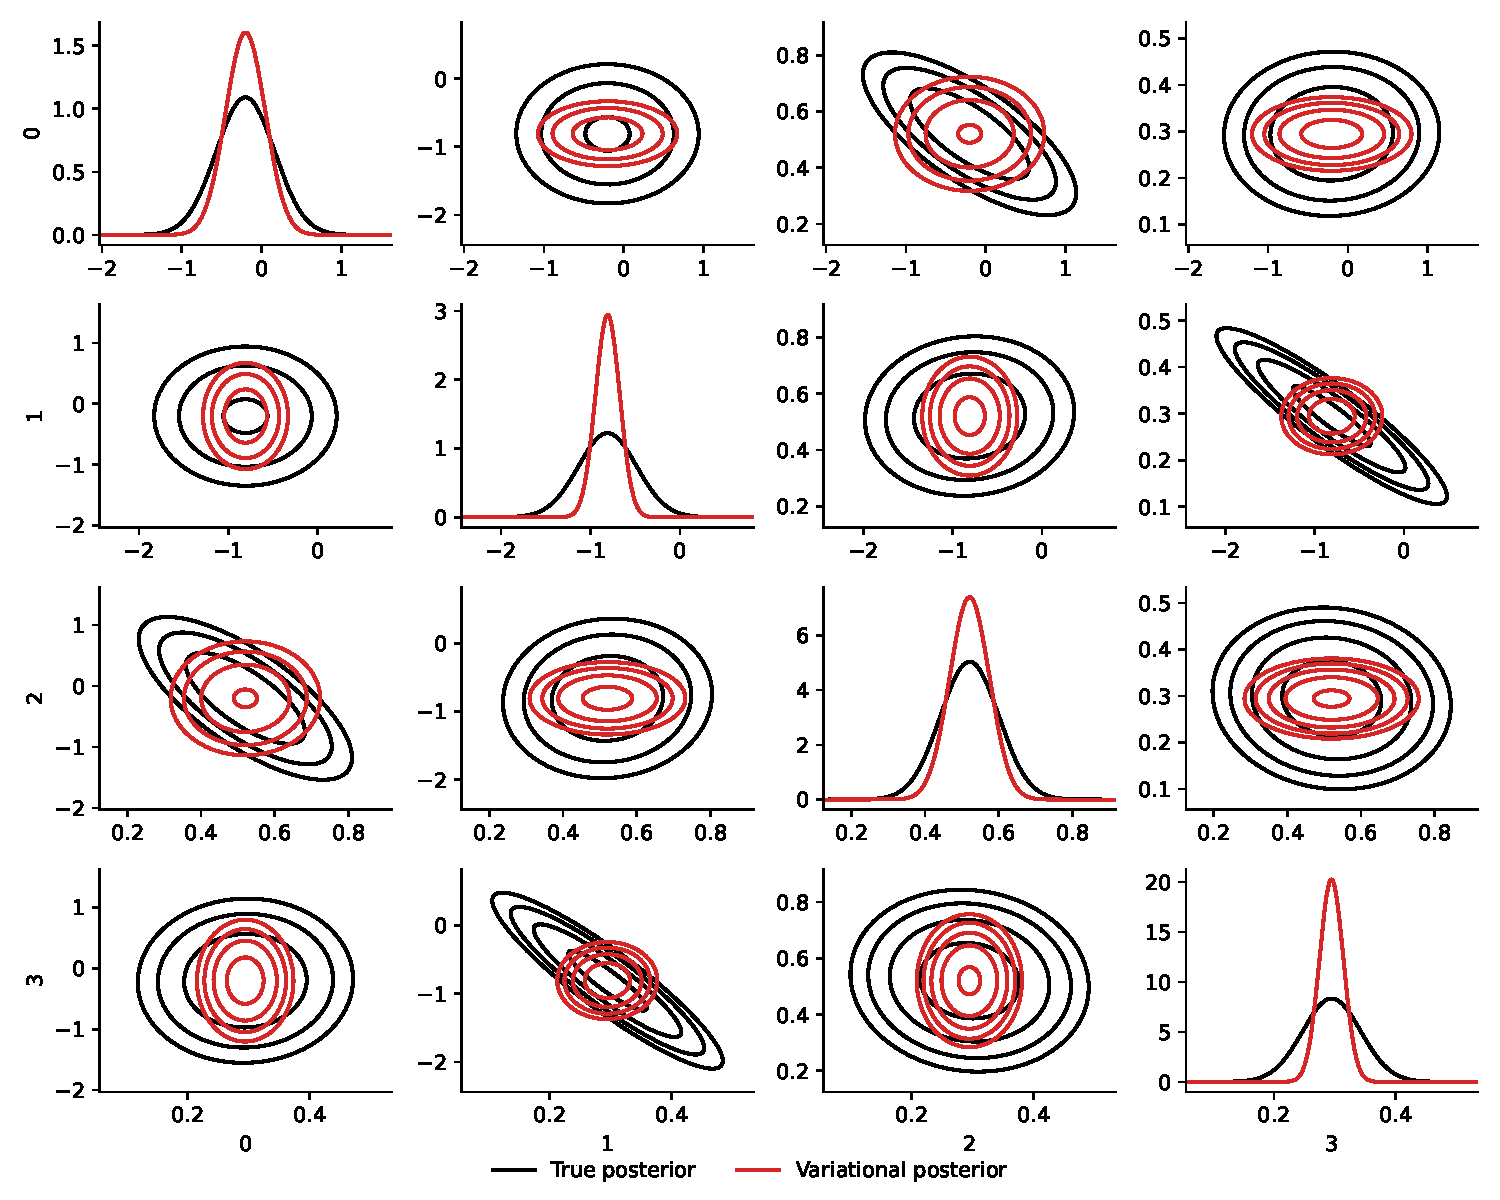
\includegraphics[width=\linewidth]{Figures/vi-simulated.pdf}
    \caption{Variational posterior compared to true posterior.}
    \label{fig:vi-simulated}
\end{figure}


\section{Estimating the variance}

In the SGHMC paper, they propose estimating the variance introduced through batching as $\hat{V}=0$, and then relying on the known simulated noise to make the inaccuracy of this estimate irrelevant. 
However, it seem to be worth investigating whether we could improve performance by providing some sort of estimate. 
This is also mentioned in the paper, however they do not seem explore the idea any further. 

Since we use an upper bound $C$ on the noise variance, parameterized by $\alpha$, we may end up with estimated noise larger than the upper bound.
Adjusting the upper bound $C$ to accommodate this, would also require adjusting the $\alpha$ parameter accordingly.
Since the $\alpha$ corresponds to the momentum decay of the algorithm, we may end up with very unstable behavior, especially for $\alpha > 1$. 
Instead, we keep $\alpha=\epsilon M^{-1}C$ fixed, and adjust the mass matrix $M$, implicitly adjusting $C$ as well.
With $M = M_0 W$ were $W$ is a diagonal matrix of weights, we can then, depending on the variance estimate, rescale the mass such that the upper bound $\alpha$ is sufficiently above the estimate $\hat\beta$, eg. by some factor $m_{\text{est}}$.
If we let the learning rate be given as $\eta_0$  for the unscaled mass matrix with $W = I$, then the learning rate for the scaled system can be found as $\eta = \epsilon^2 M^{-1} = \epsilon^2 M_0^{-1}W^{-1} = \eta_0 W^{-1}$, and
\begin{align}
    m_{\text{est}} \cdot \hat{\beta}  &\leq \alpha \Leftrightarrow\\ 
    m_{\text{est}} \cdot \frac{1}{2} \hat V \eta   &\leq \alpha \Leftrightarrow\\ 
    m_{\text{est}} \cdot \frac{1}{2} \hat V \eta_0 W^{-1}  &\leq \alpha \Leftrightarrow\\ 
    m_{\text{est}} \cdot \frac{1}{2\alpha} \hat V \eta_0   &\leq W \impliedby \\
    W_{i,i} &= \begin{cases}
        1 & \frac{1}{2\alpha}m_{\text{est}} \eta_0 \hat{V}_{i,i} < 1 \\
        \frac{1}{2\alpha}m_{\text{est}} \eta_0 \hat{V}_{i,i} & \text{otherwise}
    \end{cases}
\end{align}

The sampler then every once in a while, eg. every 50 samples, rescales the system based on the variance estimates.
If the variance estimates $\hat \beta$ happen to be greater than $\alpha$ in between the mass rescaling, the estimate is simply clamped at the upper bound $\alpha$, and no additional noise is generated.  

This method of rescaling the mass matrix is in a sense similar to the approach outlined in \cite{wenzel_how_2020}, where they also include a step calculating a preconditioning matrix, ie.
They found that using the preconditioning step generally improved performance.

There are multiple ways to go about obtaining a variance estimate.
We could try to calculate a running variance statistic using the within batch sample variance of the gradients:
\begin{equation}
    \frac{1}{|\tilde{\D}|-1}\sum_{(x_i,y_i)=\tilde{\D}} (\nabla U(\theta; x_i, y_i) - \nabla \bar{U}(\theta))^2
\end{equation}
and then scale the variance up to the fit the batch size. 
The main issue with this approach is that calculating the gradient for each observation individually within a batch is not that efficient.
While it may be possible to calculate the statistic above using autograd without doing a backward pass for each observation, it is not trivial to do so since autograd only allows for calculating gradients of scalars. 

Instead we look at three other approaches. 
The first approach is to run through a few training batches at the start of each epoch, calculating the gradient for each batch keeping the parameters constant. 
This estimate can then be used for the remaining epoch. 
The two other approaches instead keeps track of running statistics. 
The first uses exponentially decaying running estimates of the first to moments, $m_t, v_t$ as in the ADAM algorithm \cite{kingma_adam_2017}.
Since the ADAM algorithm doesn't center the second moment estimate, the squared mean is subtracted, so that the variance is estimated as $v_t - m_t^2$.

Finally, we also try to estimate the variance as with the ADAM algorithm, however using the first moment to center the second moment estimate. 

\todo{algorithme}

In order to test these three different approaches, they are applied to the simulated example from the previous section.
Every 10 sample, the variance of the gradient is estimated using 100 random batched from the training data set.
This estimate is then compared to the estimate.
The estimation provided by the estimators compared to the observed variance can be seen in \cref{fig:est_variances_simulated}.
\begin{figure}[htbp]
    \centering
    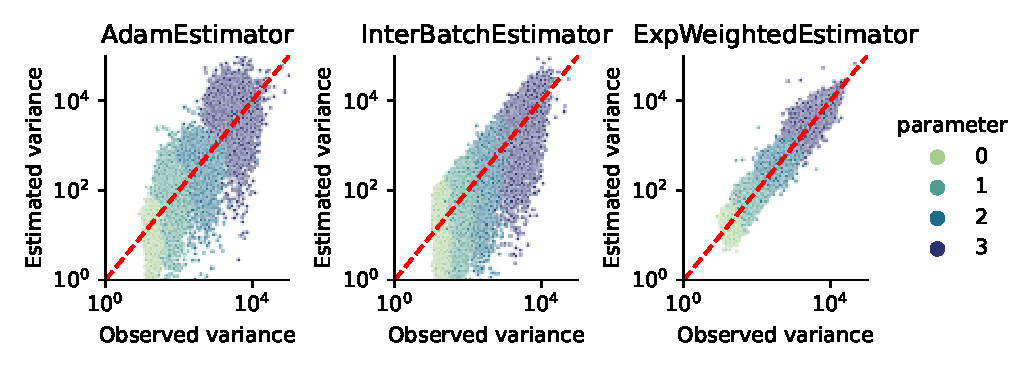
\includegraphics[width=\linewidth]{Figures/simulated_sghmc_gradient_variance_estimations.pdf}
    \caption{Estimated variance compared to observed variances}
    \label{fig:est_variances_simulated}
\end{figure}
\begin{table}[htbp]
    \centering
    \begin{tabular}{lrrrr}
\toprule
parameter &    0 &    1 &    2 &    3 \\
variance\_estimator   &      &      &      &      \\
\midrule
AdamEstimator        & 0.65 & 2.03 & 1.67 & 2.98 \\
ConstantEstimator    & 1.00 & 1.00 & 1.00 & 1.00 \\
ExpWeightedEstimator & 0.30 & 0.41 & 0.42 & 0.49 \\
InterBatchEstimator  & 1.00 & 0.98 & 0.98 & 0.94 \\
\bottomrule
\end{tabular}

    \caption{Relative errors for the different estimation schemes,}
\end{table}
Note that these values are plot using a logarithmic scale, so the estimates may seem better than they actually are, especially with when it comes to overestimating. 
It may still be that they are better than simply setting $\hat\beta=0$ in terms of estimating the posterior correctly.
In \cref{fig:simualted_var_est_joint_comp}, the sampled marginal distribution of $a_1$ and $a_3$ are shown again, now compared SGHMC with and without a variance estimator.
\begin{figure}[htbp]
    \centering
    \begin{subfigure}[t]{0.45\linewidth}
        \centering
        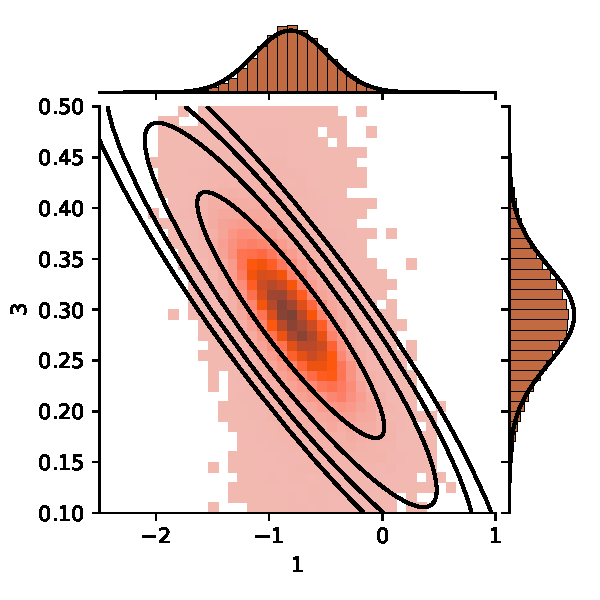
\includegraphics[width=\linewidth]{Figures/simulated_joint_SGHMC_5.pdf} 
        \caption{SGHMC with with gradient variance estimated as $\hat{V}=0$.}
    \end{subfigure}
    \begin{subfigure}[t]{0.45\linewidth}
        \centering
        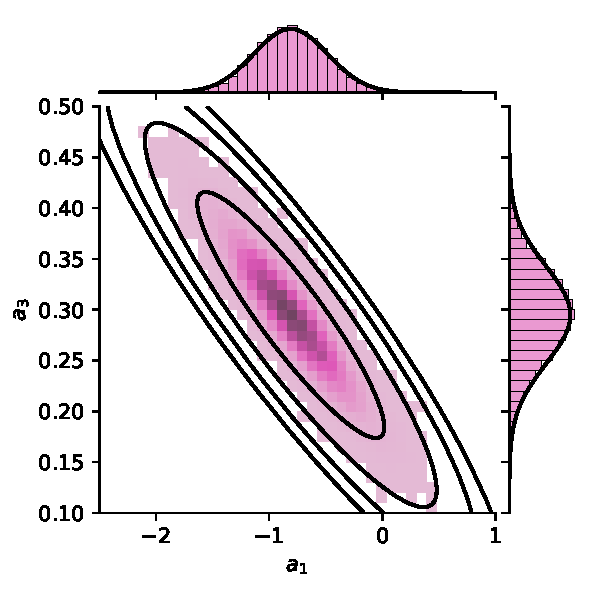
\includegraphics[width=\linewidth]{Figures/simulated_var_est_joint_ExpWeightedEstimator.pdf} 
        \caption{SGHMC with using the exponentially scaled estimator of gradient variance}
    \end{subfigure}
    \caption{Joint distribution of samples for $a_1$ and $a_3$ for the polynomial regression example for HMC and SGHMC for different batch sizes, with the actual posterior density also shown.}
    \label{fig:simualted_var_est_joint_comp}
\end{figure}
In this case, it does indeed seem like estimating the variance is able to improve the accuracy of the the sampler.
This may come down to the approach with estimated variance is able to adjust the step size down, lowering discretization and batch error compared to SGHMC without an estimator. 

\subsection{Marginal distribution of momentum}

In \cite{wenzel_how_2020}, they propose using the marginal distribution of the momentum as a test of the sampling assumptions. 
Per the dynamical system, if the system is simulated exactly, the marginal distribution of $r$ should be $\mathcal{N}(0, M^{-1})$. 
We should therefore have that $r M^{-1/2} \sim \mathcal{N}(0, I)$. 
Applying the inner product, we arrive at so called kinetic temperature $T_K(r) = \frac{r^T M r}{d}$, for which we then have that $T_K(r)d\sim \chi^2(d)$, where $d$ is the length of $r$ ie. the number of parameters. 
We then consider some $c\in (0, 1)$ confidence interval of  $\chi^2(d)$ distribution:
\begin{align}
    J_{T_k}(d, c) = \left(\frac{1}{d} F_{\chi^2(d)}^{-1}\left( \frac{1-c}{2} \right),~\frac{1}{d} F_{\chi^2(d)}^{-1}\left(\frac{1+c}{2}\right)\right),
\end{align}
where $F_{\chi^2(d)}^{-1}$ is the inverse cumulative distribution function of the $\chi^2(d)$ distribution.
We would expect the samples for $\hat{T}_K$ to fall within the interval $J_{T_k}(d, c)$ with probability exactly $c$. 
We should therefore expect $\E[\hat{T}_K \in J_{T_K}(d, {0.99})] = 0.99$ given a perfectly simulated system.
This allows us to test the correctness of our sampler, even if we don't know the true posterior, which is going to be the case in the following experiments.

Applying this statistic, we can see whether the estimation of the variance helps with regard to the correctness of the simulation. 
Returning back to our simulated polynomial example, in the previous experiment, the momentum were resampled every $10$ epochs, to make to comparison to regular HMC as clear as possible. 
However, if we resample the momentum from the marginal distribution too often, the $\hat{T}_{0.99}$ measure would obviously be less informative with regard to the influence of discretization and batching error. 
The momentum is therefore instead resampled every $1000$ steps, with a slightly lower learning rate of $\eta=4 \cdot 10^{-5}$.
The lower learning rate is used since otherwise, the SGHMC sampler with $\hat{\beta}=0$ becomes unstable. 
\begin{figure}[htbp]
    \centering
    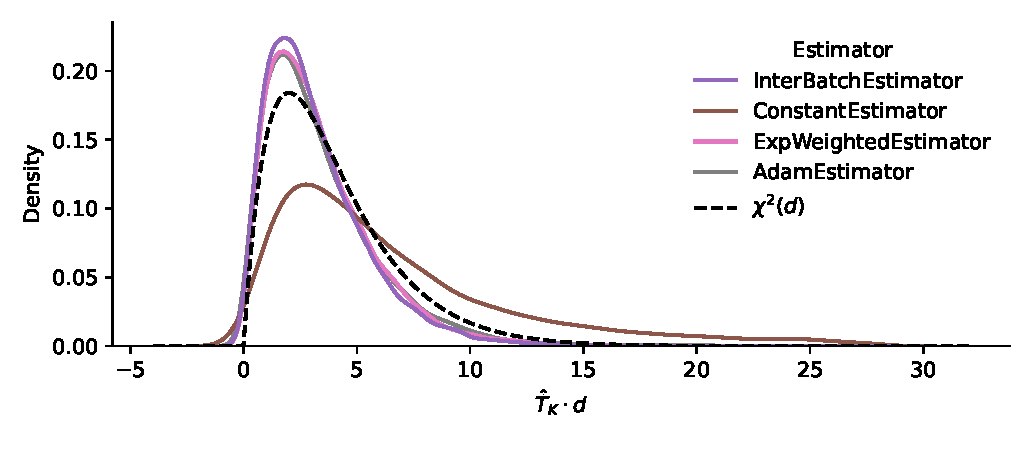
\includegraphics[width=\linewidth]{Figures/temperature_sum_chi2_comp.pdf}
    \caption{<0 is because of the KDE approdiximation...}
    \label{fig:temperature_sum_chi2_comp}
\end{figure}

\begin{table}[htbp]
    \centering
    \begin{tabular}{lc}
\toprule
           Estimator & $\E[\hat{T}_K \in J_{T_K}(d, {0.99})]$ \\
\midrule
       AdamEstimator &                    $98.65 \pm 0.18~\%$ \\
   ConstantEstimator &                    $85.75 \pm 0.54~\%$ \\
ExpWeightedEstimator &                    $99.15 \pm 0.14~\%$ \\
 InterBatchEstimator &                    $99.01 \pm 0.15~\%$ \\
\bottomrule
\end{tabular}

    \caption{<caption>}
    \label{tbl:temp_99}
\end{table}
The resulting distribution of $\hat{T}_K$ can be seen in \cref{fig:temperature_sum_chi2_comp}, compared against the expected $\chi^2$ distribution. 
We see that the while the samplers with estimated variance doesn't fit the distributional assumptions, they are all much closer than the for the sampler with $\hat \beta = 0$.
The $\hat T_{0.99}$ statistic have also been calculated in \cref{tbl:temp_99}, alongside a confidence interval based on the binomial distribution.

It seem like the samplers with estimated variance are all underdispersing slightly, compared to the actual posterior. with  which would make sense if we are overestimating variance.
Looking at the PLOT, the estimation margin estimates also seems relatively uniformly distributed on the log scale, which would mean that we are generally overestimating with larger magnitude. 
Since we are overestimating the noise from batching, this would lead to us not adding sufficient noise to the system, leading to underdispersion.

\section{MNIST}
In this section, we will explore the performance of the different methods on the MNIST dataset for classification. 
This dataset is often used to benchmark and compare different methods and implementations. 

In \cite{chen_stochastic_2014} they also compare against MNIST, using a small neural network with a single hidden layer of 100 units.
For this model, they demonstrate comparable, and even superior performance compared to SGD methods using weight regularization.
The authors of \cite{blundell_weight_2015} also compare with MNIST, only they use much larger networks with two hidden layers of size 400, 800 and 1200. 
They also compare against regular SGD, also using dropout during training, showing slightly better test performance of VI.

In this project, we compare all these methods using a regular feed forward neural network with two hidden layers of size 800 and using ReLU as activation function. 
We will be using a batch size of 128 for the optimization based algorithms and 500 for the MCMC algorithms.
Further, for the MCMC algorithms, we are keeping a sample for every epoch, after a burn in period of 50 epochs.
The different algorithms all have some number of  hyperparameters that can we can tune, some algorithms more than others.
In an effort to keep the comparison fair between the algorithms, the hyperparameter optimization framework Optuna \cite{akiba_optuna_2019} is used. 
This framework treats the choice of hyperparameters as a black box optimization problem, trying to figure out what choices of parameters leads to the best validation error.

Another modelling choice is the question of parameter priors for the probabilistic methods. 
For the MCMC method we choose a hierarchal prior as in \cite{chen_stochastic_2014}. 
For each parameter group $\Theta_i=\{\theta_{i,1},\dots,\theta_{i,D_i}\}$, such as the bias or weight of some linear layer , we then use a Gaussian prior for the parameters $\theta_{i,j} \sim  \mathcal{N}(0, \sigma_i^2)$.
We then choose an uninformative prior for the variance parameters $1/\sigma_i^2 = \lambda_i \sim \Gamma(1,1)$.
This enables different parameter groups to have parameters on different scales.
In the MCMC framework, we are able to sample the precision parameters through a Gibbs step, using the conjugate distribution $p(\lambda_i | \Theta_i)$.
This allows us to sample from parameter posterior conditioned on the precision using SGHMC and then update the precision $p(\lambda_i | \Theta_i)$.

Since we are not able to a Gibbs step during the non-MCMC methods, we instead use a mixture of two Gaussian distributions,
\begin{align}
    \theta \sim t\cdot \mathcal{N}(0, \sigma_1^2) + (1-t)\cdot \mathcal{N}(0, \sigma_2^2),
\end{align}
as prior as proposed in the \cite{blundell_weight_2015}.
This allows for greater flexibility than a simple Gaussian, while not requiring us to optimize the prior of variance parameters as well.
The parameters for the mixture prior will be found through hyperparameter search.

For each algorithm, we spend 24 hours to figure out sensible values for the various hyperparameters over 1000 epochs. 
Since the variational method may be a lot slower than the other methods if using a lot of samples for estimating the ELBO gradient, we impose a 2 hour time limit for each training run. 
For each algorithm, the hyperparameters are then set based on the top few results and the models are trained a final time.
The validation curves corresponding to each training run for each algorithm can be seen in \cref{fig:mnist-best-val-curves}.
\begin{figure}[htbp]
    \centering
    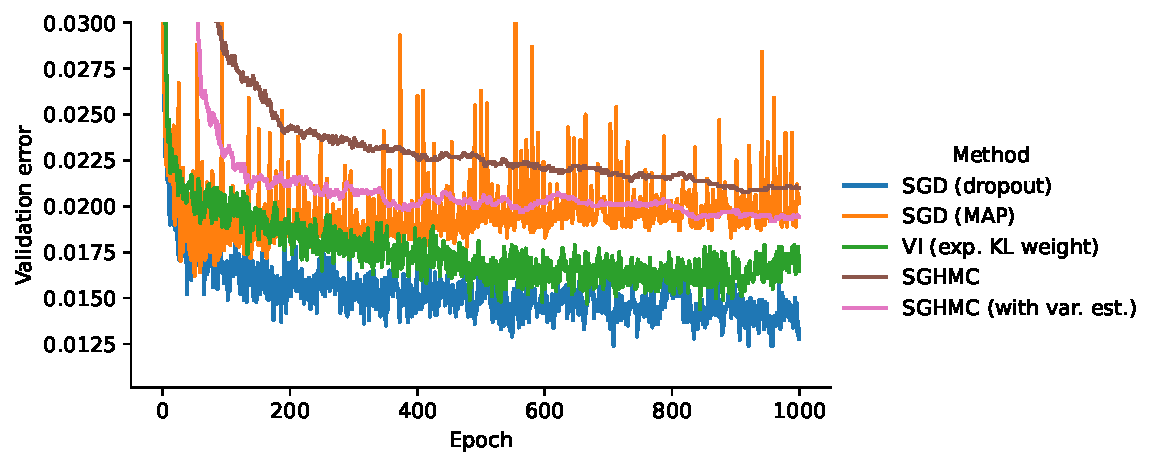
\includegraphics[width=\linewidth]{Figures/mnist-final-runs-val.pdf}
    \caption{Validation curves for final training runs for each algorithm.}
    \label{fig:mnist-best-val-curves}
\end{figure}
Tables documenting the choice of parameters can be seen in \cref{apx:mnist-sweep}.
We choose to use the scheduled re-weighting of the KL-term for the VI algorithm, as we see it performing better than using the constant weight.

Seeing as some of the algorithms tended to overfit, the best model during training according to validation error is chosen for the non-MCMC methods.
The variational algorithm is given some more time to finish training, to see whether the performance increases if we let the model train for all 1000 epochs. 
The resulting testing errors for each algorithm can be seen in \cref{tab:mnist-test-err}.
\begin{table}[htbp]
    \centering
    \begin{tabular}{ll}
\toprule
{} & Test error incl. 95\% CI \\
\midrule
SGD (MAP)              &      $0.0175 \pm 0.0026$ \\
SGD (dropout)          &      $0.0143 \pm 0.0023$ \\
SGHMC                  &      $0.0173 \pm 0.0026$ \\
SGHMC (with var. est.) &      $0.0158 \pm 0.0024$ \\
VI                     &       $0.0243 \pm 0.003$ \\
\bottomrule
\end{tabular}

    \caption{Testing errors for MNIST for different inference algorithm.}
    \label{tab:mnist-test-err}
\end{table}
We see that out of the methods attempted, regular SGD with dropout wins out, however not by a lot. 
Interestingly, both SGHMC methods seem to perform a significantly better than suggested by the validation error curves. 
Since we used the validation set for tuning our parameters, we would in fact expect the opposite to be true. 
In any case, both the validation and test error seems to indicate that the SGHMC using gradient variance estimation improves the predictive performance of the models.

\subsection{Calibration}

As mentioned in the introduction, poorly calibrated inference is not uncommon with complex machine learning models. 
A key motivator for experimenting with Bayesian methods has been to try and get a more robust and reliable estimate.
As in \cite{guo_calibration_2017} we use the \emph{expected calibration error} (ECE) for benchmarking the uncertainty of the different methods.
For some set of predictions, $\hat{y}$ the \emph{confidence} is defined as the estimated probability $\hat{p}$ of belonging to the estimated class.
The ECE statistic compares the confidence of the model to the observed accuracies.
This is done by first grouping the test observations into $M$ bins of size $1/M$, according to the output confidence. 

Then, the accuracy of each bin $B_m$, can be calculated as:
\begin{align}
    \acc(B_m) = \frac{1}{|B_m|}\sum_{i\in B_m}\bm{1}(\hat{y}_i = y_i)
\end{align}
Likewise, we calculate the average model confidence across the bin
\begin{align}
    \conf(B_m) = \frac{1}{|B_m|}\sum_{i\in B_m} \hat{p}_i.
\end{align}
Now, if the confidence of the model is to be trusted, we would expect $\acc(B_m) = \conf(B_m)$.
These measures thus gives us a way to benchmark the uncertainty of the model.
We then calculate the ECE as the expected absolute difference between the accuracy and the confidence weighted according to the size of each bin
\begin{align}
    \text{ECE} = \sum_{m=1}^{M} \frac{|B_m|}{n}|\acc(B_m)-\conf(B_m)|.
\end{align}
This gives us a single statistic to compare the inference methods across.
In \cref{tab:mnist-ece}, the ECE for the test set can be seen for each of the inference methods.
The accuracy and mean confidence of each bin can be seen in \cref{fig:mnist-calibration}. 
\begin{table}[htbp]
    \centering
    \begin{tabular}{lr}
\toprule
{} &   ECE \\
\midrule
SGD (dropout)          & 1.39\% \\
SGD (MAP)              & 1.00\% \\
VI (exp. KL weight)    & 0.77\% \\
SGHMC                  & 3.04\% \\
SGHMC (with var. est.) & 1.55\% \\
\bottomrule
\end{tabular}

    \caption{ECE on test set for models trained on the MNIST dataset.}
    \label{tab:mnist-ece}
\end{table}
\begin{figure}[htbp]
    \centering
    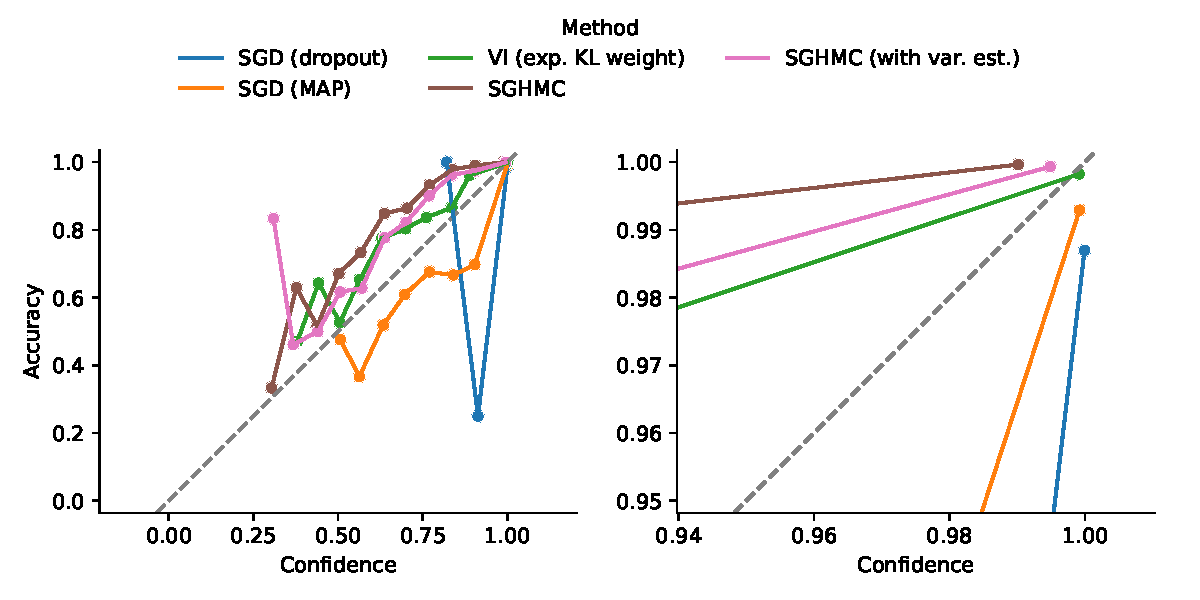
\includegraphics[width=\linewidth]{Figures/mnist-calibration.pdf}
    \caption{Accuracy and mean confidence across different bins for each algorithm.}
    \label{fig:mnist-calibration}
\end{figure}
We see that the VI is the best performing algorithm with respect to ECE, while the MCMC algorithms are the worst performers. 
Compared to the SDG based algorithms, there doesn't seem to be a clear advantage to applying the probabilistic methods.

\subsection{Checking SGHMC Assumptions}
As with the polynomial model, we can use the marginal distribution of the momentum variables $r$ to examine how well the sampled distribution resembles the correct distribution.
For each parameter group, the corresponding 0.99 $\chi^2$ quantile has been calculated, and \cref{tab:mnist-temperatures} show the observed fraction of samples falling within the quantile, $\hat{T}_{0.99}$.
\begin{table}[htbp]
    \centering
    \begin{tabular}{ll}
\toprule
               Sampler &    $\hat{T}_{0.99}$ \\
\midrule
                 SGHMC & $66.67 \pm 0.84~\%$ \\
SGHMC (with var. est.) & $67.07 \pm 0.84~\%$ \\
\bottomrule
\end{tabular}

    \caption{Observed values of $\hat{T}_{0.99}$ for MNIST model.}
    \label{tab:mnist-temperatures}
\end{table}
A graph showing the observed distribution compared the expected distribution for each parameter group can be seen in \cref{fig:mnist-temperatures}. 
We see that samples from neither of the sampling methods matches the correct marginal distribution for the momentum variables. 
It therefore seems like the sampling methods breaks down for many parameters compared to the simple examples explored in the previous experiments.

It is worth noting, that we optimized the choice of hyperparameters with respect to the validation error, which does not necessarily imply correctness of the samples from the posterior. 
\begin{figure}[htbp]
    \centering
    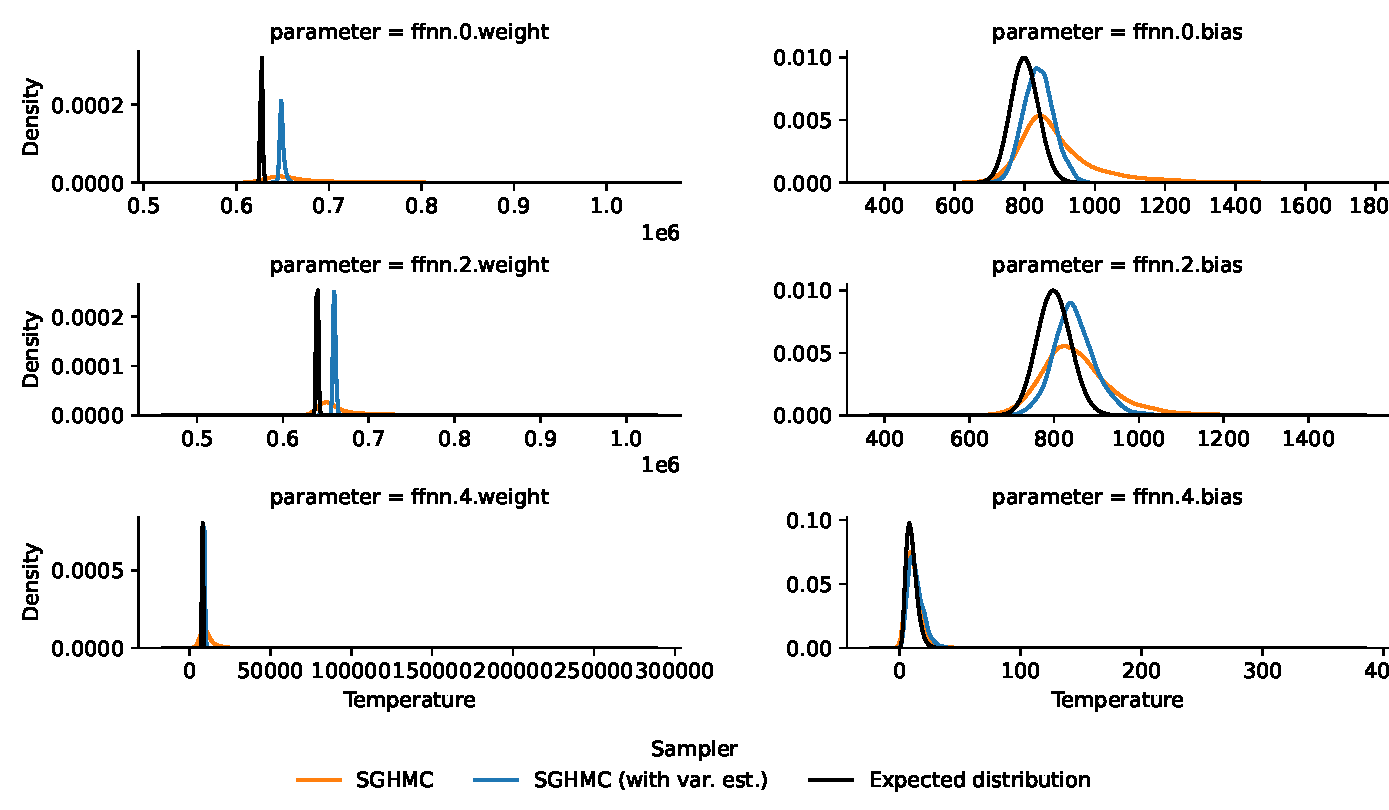
\includegraphics[width=\linewidth]{Figures/mnist-temperatures.pdf}
    \caption{Temperature distributions for different parameter groups in the model during SGHMC training.}
    \label{fig:mnist-temperatures}
\end{figure}

\FloatBarrier
\section{Convolutional Neural Network}

While the combination of MNIST and feed forward neural networks is used as a baseline by many, it is not the most representative example of advanced image analysis techniques.
In the following section, we will investigate the performance of the different methods using a convolutional neural network (CNN) model, as well as benchmarking against the more difficult CIFAR-10 dataset.

We initially attempt to fit a smaller CNN from scratch.
This model consist of 3 convolutional layers, each with 4o channels and a kernel size of 5.
Each convolution is following by a batch normalization layer, a ReLU activation function and a max pooling layer.
These layers are then followed by a single linear layer of size 256, leading out to the output.

The batch normalization layers are shown to improve training performance by reducing internal covariate shift.
Due to the running moment estimates of the batch normalization layers, the probabilistic interpretation of becomes less clear, and we therefore only include them for the models trained with dropout. 

For the sampling methods, we again use a burn in period of 50 epochs.
Instead of keeping a sample for every epochs, we now retain up to 200 samples.
This is done in a roughly uniform manner, dynamically increasing the number of epochs between samples while pruning already retained samples.
We are using the same batch sizes as in the previous experiment.

We run hyperparameter search as with the previous experiment, however now searching for 12 hours combined with an early stopping criteria.
This means that during training, if no improvement has been seen with respect to validation error for 15 epochs, we finish the experiment and try another value.
Based on the hyperparameters with the best performance, the parameters seen in \cref{tab:cifar10-small-hparams} is chosen, and the model is trained again. 
The hyperparameter search for the two SGHMC methods doesn't really show clear cut choices for either algorithm, and we therefore prioritize setting the same parameters across both methods for comparison. 
\begin{table}[htbp]
    \centering
    \begin{tabular}{p{4cm}p{9cm}}
        \toprule
        Algorithm & Parameters chosen \\ \midrule
        SGD (MAP) & 
        $\texttt{lr}=9 \times 10^{-4}$, 
        $\log\sigma_1=-2$, 
        $\log\sigma_2=-8$, 
        $\texttt{mixture\_ratio}=0.6$ \\ \midrule
        SGD (dropout) & $\texttt{lr}=9\times 10^{-4}$,
        $\texttt{dropout}=0.6$ \\ \midrule
        SGHMC & $\texttt{lr}=2\times 10^{-7}$, $\alpha=0.05$, \texttt{resample\_momentum\_every}=10000 \\ \midrule
        SGHMC (with variance estimate) &  $\texttt{lr}= 2 \times 10^{-7}$, 
        $\alpha=0.05$,
        $\texttt{estimation\_margin}=2$, \texttt{resample\_momentum\_every}=10000 \\  \midrule
        Variational inference &    
        $\texttt{lr}=5 \times 10^{-4}$,
        $\log\sigma_1=-1$,
        $\log\sigma_2=-8$,
        $\texttt{mixture\_ratio}=0.35$,
        $\texttt{n\_particles}=7$, constant KL weight \\
        \bottomrule
    \end{tabular}
    \caption{Chosen hyperparameters for small CIFAR10 model.}
    \label{tab:cifar10-small-hparams}
\end{table}
For each method, the validation curves during the final training run can be seen in \cref{fig:cifar-small-final-runs-val}, and the resulting testing errors can be seen in \cref{tab:cifar10-small-test-err}.
\begin{figure}[htbp]
    \centering
    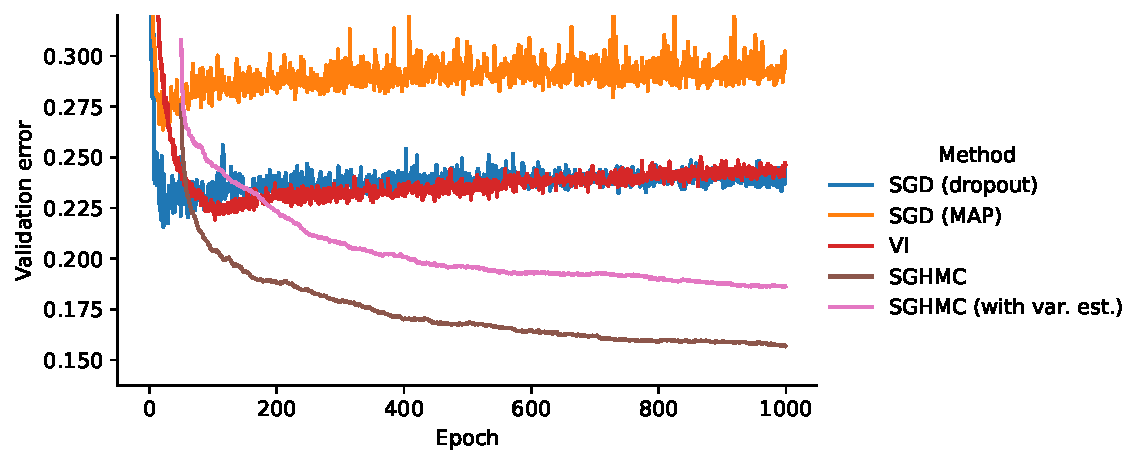
\includegraphics[width=\linewidth]{Figures/cifar-small-final-runs-val.pdf}    
    \caption{<caption>}
    \label{fig:cifar-small-final-runs-val}
\end{figure}
{tab:cifar10-small-test-err}. 
\begin{table}[htbp]
    \centering
    \begin{tabular}{ll}
\toprule
{} & Test error incl. 95\% CI \\
\midrule
SGD (MAP)              &      $29.28 \pm 0.89~\%$ \\
SGD (dropout)          &      $24.88 \pm 0.85~\%$ \\
SGHMC                  &      $16.57 \pm 0.73~\%$ \\
SGHMC (with var. est.) &      $19.02 \pm 0.77~\%$ \\
VI                     &      $24.90 \pm 0.85~\%$ \\
\bottomrule
\end{tabular}

    \caption{Test error for small convolutional model on CIFAR10 dataset}
    \label{tab:cifar10-small-test-err}
\end{table}
Here we see the MCMC methods clearly outperform the other methods.
Of the two MCMC methods, the regular SGHMC without gradient variance estimation achieves better test error. 

This may partly be because of how the early stopping criteria.
As we can see in the \cref{fig:cifar-small-final-runs-val}, the validation error is characterized by some variance.
This may lead to relatively large occasional one-time decreases in validation error, resulting in the early stopping criteria stopping prematurely.
This favors strategies with good initial increase in performance, however may unfairly disfavor slower strategies that may lead to better performance over time.

Another point relating to the fairness of comparing the methods, is that the MCMC methods are predicting based on a far larger ensemble of different models.
Investigating the effect of the ensemble methods, we uniformly, without replacement sample anywhere from 1 up to and including every sample from the MCMC ensemble, and measure the test performance as function of the size of the ensemble. 
\begin{figure}[htbp]
    \centering
    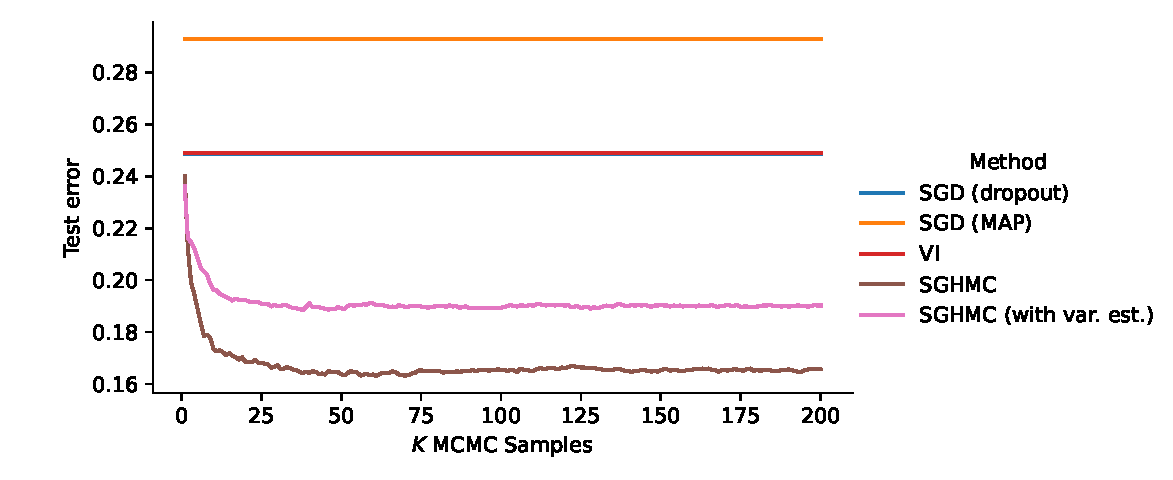
\includegraphics[width=\linewidth]{Figures/cifar-small-downsampling.pdf}
    \caption{Test performance for MCMC methods as a function of the size of the model ensemble.
The test performance of the other methods are shown as horizontal lines for comparison.
Due to very similar test errors, the line corresponding to SGD with dropout is hidden underneath the line for VI.}
    \label{fig:cifar-small-downsampling}
\end{figure}
The corresponding curves can be seen in \cref{fig:cifar-small-downsampling}.
Here we see that the performance is not really that dependent on the sample size after $\approx 50$ samples, and even with only a single sample, both SGHMC algorithms are performing better than the others.

\subsection{Calibration}
As in the experiment, we also measure the ECE on the test set, to evaluate how well calibrated the models are.
The estimates can be seen in \cref{tab:cifar-small-ece}.
\begin{table}[htbp]
    \centering
    \begin{tabular}{lr}
\toprule
{} &    ECE \\
\midrule
SGD (dropout)          & 21.87\% \\
SGD (MAP)              & 18.47\% \\
VI                     &  3.62\% \\
SGHMC                  &  7.55\% \\
SGHMC (with var. est.) &  6.54\% \\
\bottomrule
\end{tabular}

    \caption{ECE for small convolutional model on the CIFAR10 dataset.}
    \label{tab:cifar-small-ece}
\end{table}
Here we see the probabilistic methods are does seem to be better calibrated than the SGD methods.
VI again results in the best calibrated model, now by some margin.
If we take a look at \cref{fig:cifar-small-calibration} we also see that while the SGD method are generally way overconfident, the probabilistic methods tend to be underconfident.
\begin{figure}[htbp]
    \centering
    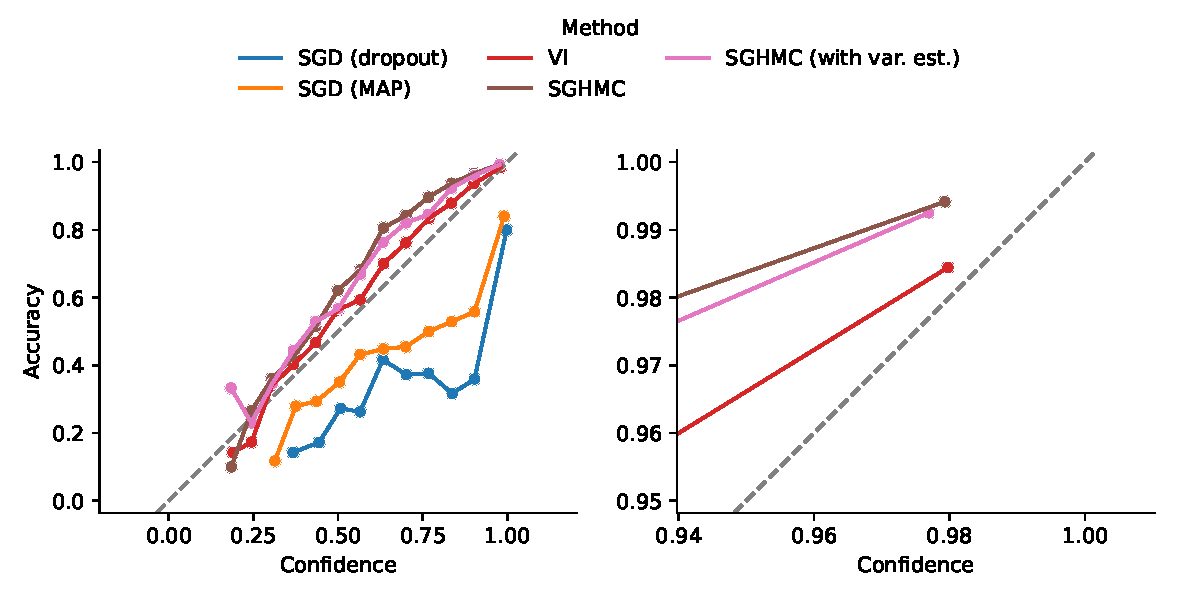
\includegraphics[width=\linewidth]{Figures/cifar-small-calibration.pdf}
    \caption{cifar-small-calibration}
    \label{fig:cifar-small-calibration}
\end{figure}
\subsection{SGHMC Assumptions}
Again, we look at how well the distributional assumptions are met for the sampling algorithms.
In \cref{fig:cifar-small-temperatures} the observed temperatures $T$
\begin{figure}[htbp]
    \centering
    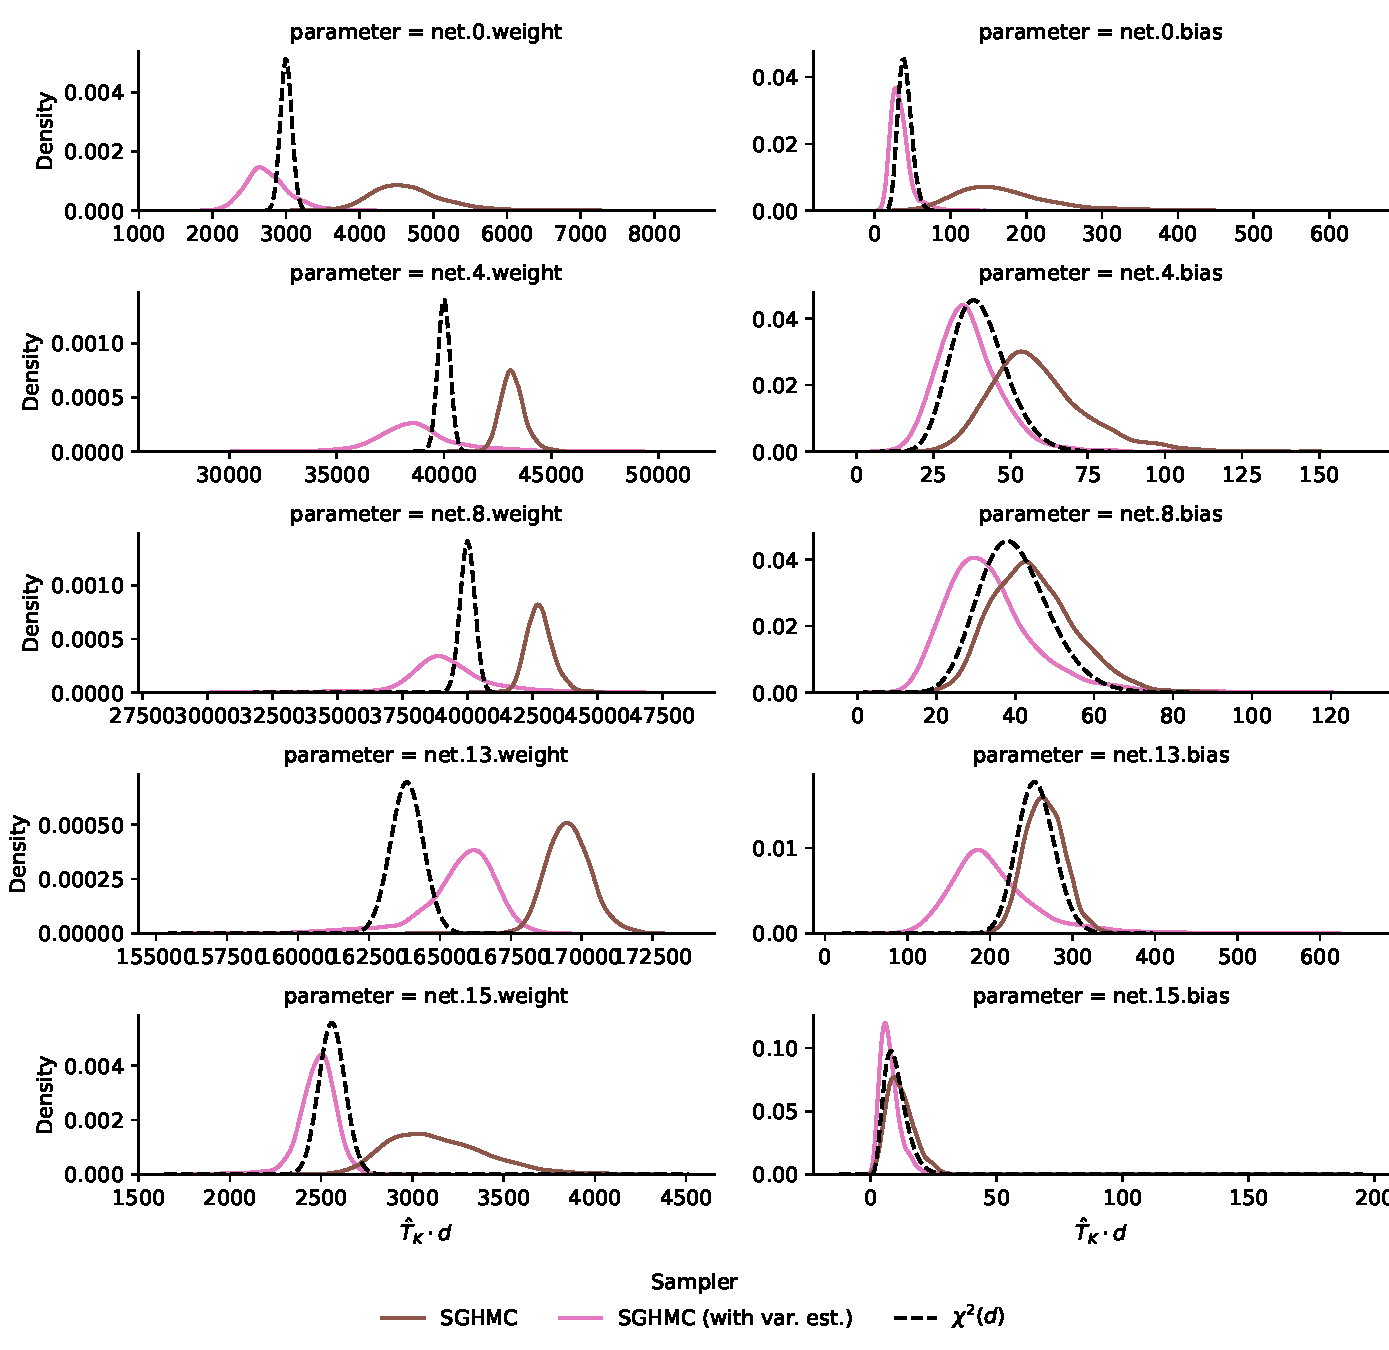
\includegraphics[width=\linewidth]{Figures/cifar-small-temperatures.pdf}
    \caption{<caption>}
    \label{fig:cifar-small-temperatures}
\end{figure}

\begin{table}[htbp]
    \centering
    \begin{tabular}{lc}
\toprule
                Method & $\E[\hat{T}_K \in J_{T_K}(d, {0.99})]$ \\
\midrule
                 SGHMC &                    37.24 $\pm$ 0.75~\% \\
SGHMC (with var. est.) &                    59.31 $\pm$ 0.76~\% \\
\bottomrule
\end{tabular}

    \caption{Observed values of $\hat{T}_{0.99}$ for small CIFAR 10 model.}
    \label{tab:cifar-small-temperatures}
\end{table}

\FloatBarrier
\section{Densenet}
Finally, we will be looking into how well the different methods handles even larger models.
As an example of a model of the larger variety, we look at training the Densenet model \cite{huang_densely_2017}.
We are 

Due to considerably larger model and training time, we are not doing a hyperparameter search like with the previous two models.
Instead we try three different learning rate with every other hyperparameter fixed.
For the SGD and VI methods, we try learning rates of $2\times 10^{-4},5\times 10^{-4},1\times 10{^-3}$, and for SGHMC we try the learning rates $2\times 10^{-8},5\times 10^{-8},1 \times 10^{-7}$.
\todo{other parameters}

Each model gets to train for up to 1000 epochs, with a limit of 7 hours training time.
For this experiment, every algorithm is trained with a batch size of 128.

it may be that the batch norm is not really important for the relatively shallow conv net.

\begin{figure}[htbp]
    \centering
    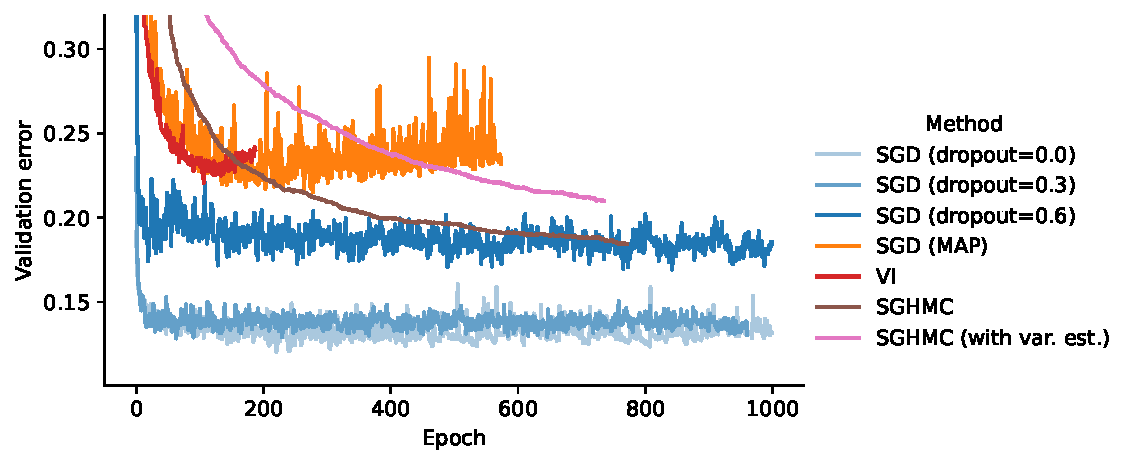
\includegraphics[width=\linewidth]{Figures/cifar-densenet-final-runs-val.pdf}
    \caption{<caption>}
    \label{<label>}
\end{figure}

\begin{table}[htbp]
    \centering
    \begin{tabular}{ll}
\toprule
                Method & Test error incl. 95\% CI \\
\midrule
             SGD (MAP) &      $23.36 \pm 0.83~\%$ \\
     SGD (dropout=0.0) &      $13.71 \pm 0.67~\%$ \\
     SGD (dropout=0.3) &      $14.01 \pm 0.68~\%$ \\
     SGD (dropout=0.6) &      $19.68 \pm 0.78~\%$ \\
                 SGHMC &      $18.96 \pm 0.77~\%$ \\
SGHMC (with var. est.) &      $21.17 \pm 0.80~\%$ \\
                    VI &      $24.32 \pm 0.84~\%$ \\
\bottomrule
\end{tabular}

    \caption{<caption>}
    \label{<label>}
\end{table}

\subsection{Calibration}

\begin{table}[htbp]
    \centering
    \begin{tabular}{lr}
\toprule
{} &    ECE \\
\midrule
SGD (MAP)              & 15.62\% \\
SGD (dropout=0.0)      & 11.14\% \\
SGD (dropout=0.3)      & 11.75\% \\
SGD (dropout=0.6)      & 16.85\% \\
SGHMC                  & 10.33\% \\
SGHMC (with var. est.) &  9.46\% \\
VI                     &  8.77\% \\
\bottomrule
\end{tabular}

    \caption{ECE for Densenet on the CIFAR10 dataset.}
    \label{tab:cifar-densense-ece}
\end{table}
Here we see a 
\begin{figure}[htbp]
    \centering
    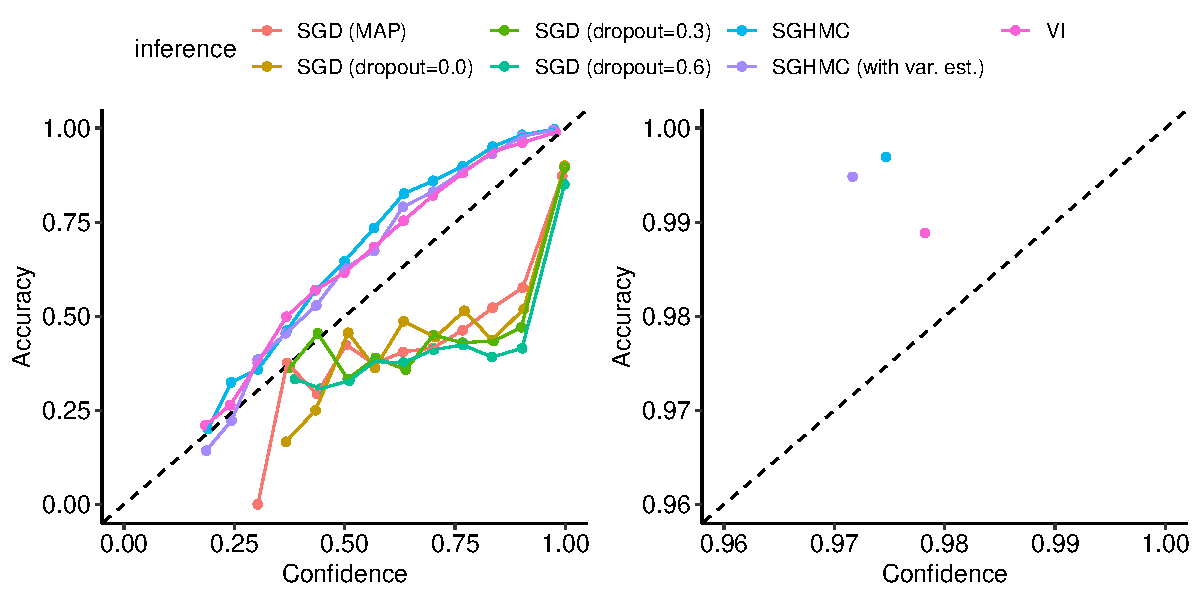
\includegraphics[width=\linewidth]{Figures/cifar10-densenet-calibration.pdf}
    \caption{<caption>}
    \label{<label>}
\end{figure}



\subsection{SGHMC Assumptions}
\begin{figure}[htbp]
    \centering
    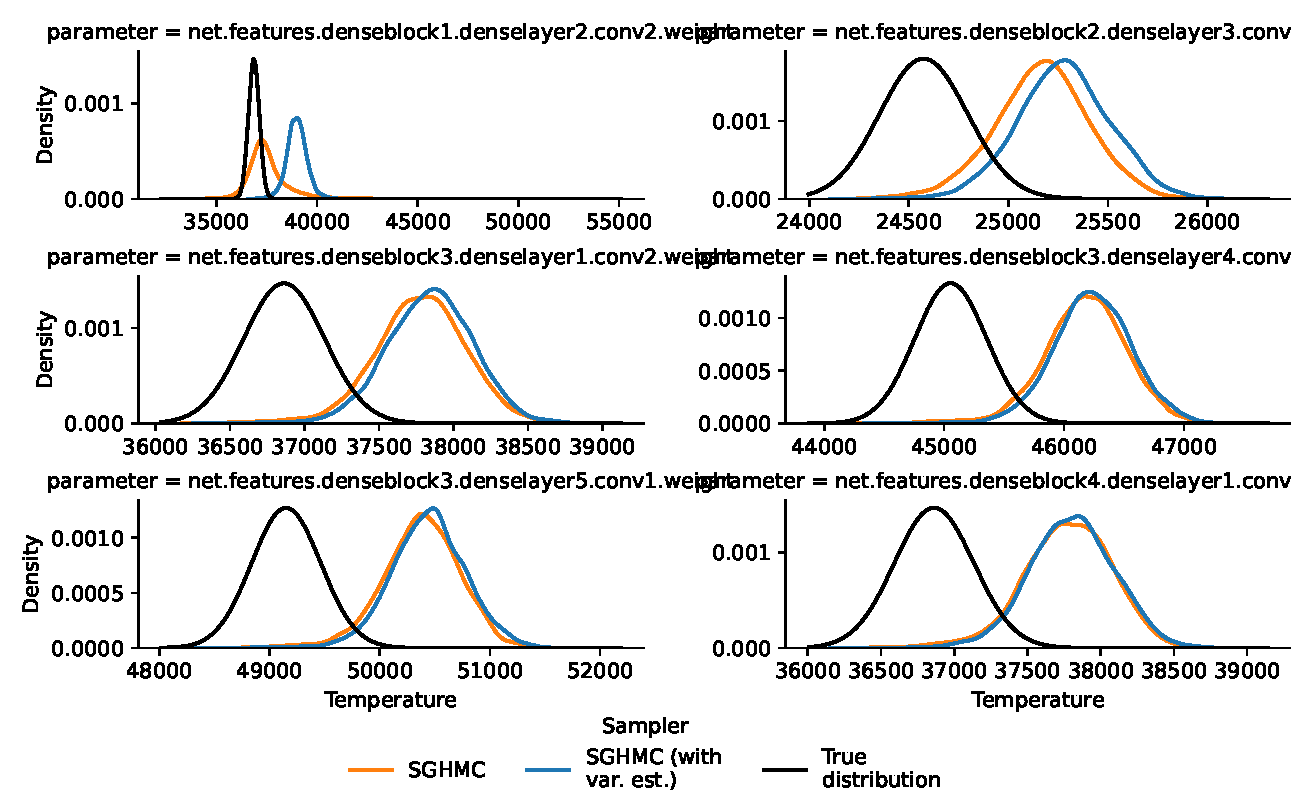
\includegraphics[width=\linewidth]{Figures/cifar-densenet-temperatures.pdf}
    \caption{<caption>}
    \label{<label>}
\end{figure}

\begin{table}[htbp]
    \centering
    \begin{tabular}{ll}
\toprule
                Method & Test error incl. 95\% CI \\
\midrule
             SGD (MAP) &      $23.36 \pm 0.83~\%$ \\
     SGD (dropout=0.0) &      $13.71 \pm 0.67~\%$ \\
     SGD (dropout=0.3) &      $14.01 \pm 0.68~\%$ \\
     SGD (dropout=0.6) &      $19.68 \pm 0.78~\%$ \\
                 SGHMC &      $18.96 \pm 0.77~\%$ \\
SGHMC (with var. est.) &      $21.17 \pm 0.80~\%$ \\
                    VI &      $24.32 \pm 0.84~\%$ \\
\bottomrule
\end{tabular}

    \caption{Observed values of $\hat{T}_{0.99}$ for small CIFAR 10 model.}
    \label{tab:cifar-densenet-temperatures}
\end{table}